		The rank of a card is determined by the numerical value in the top-left and bottom-right corners, and in the case of any card that is not a picture card, the quantity of suit symbols in the centre of the card itself. Thus, cards 2 through 10 are scored by their numerical value by the software implementation using the quantity of suit symbols.

		\subsubsection{Value cards}
			The first step in this classification stage is to convert the card image to a binary segmented form using simple thresholding, then by flood-filling the top-left and bottom-right corners, whose features are not used for value detection, as shown below:

			\begin{lstlisting}

cv::Mat temp = card->mat_bin.clone();

//Ignore the corners
cv::rectangle(temp, Card::TOP_CORNER_RECT, cv::Scalar(255), CV_FILLED);
cv::rectangle(temp, Card::BOTTOM_CORNER_RECT, cv::Scalar(255), CV_FILLED);
			\end{lstlisting}

			Once this is complete, the remaining blobs are morphologically eroded and closed to clear up the regions into single homogeneous blobs. This is done using custom morphological implementations which can be found in the source code under \source{cl\_own.cpp}{app:clowncpp}.

			\begin{lstlisting}

//Erode and close
temp = binary_operation(temp, MODE_BINARY_DILATION, 5);
temp = binary_closing(temp, 10);
			\end{lstlisting}

			The result is shown in Figure~\ref{fig:closing}:

			\begin{figure}[H]
				\centering
				\begin{subfigure}[b]{0.4\textwidth}
					\centering
					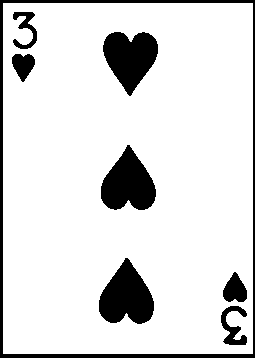
\includegraphics[width=\textwidth]{chris/image20}
					\caption{}
				\end{subfigure}
				\begin{subfigure}[b]{0.4\textwidth}
					\centering
					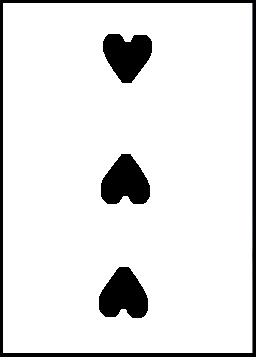
\includegraphics[width=\textwidth]{chris/image21}
					\caption{}
				\end{subfigure}
				\caption{Binary threshold segmented card with extraneous features removed}
				\label{fig:closing}
			\end{figure}

			After this, the remaining blobs are counted and filled, and is equal to the value of the card itself for the sample deck used for evaluation.

		\subsubsection{Picture cards}
			In the case of picture cards (except for the case of an Ace), there is to relationship between the number of blobs in the centre of the card and its value, such as a King. To get around this, the presence of a picture card is determined by the presence of an additional contour inside the isolated card, i.e.: there is a rectangle within the card rectangle, as illustrated below:

			\begin{figure}[H]
				\centering
				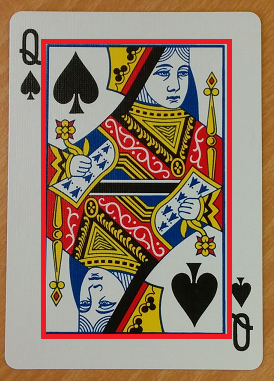
\includegraphics[width=0.4\textwidth]{chris/image22}
				\caption{A picture card such as Jack, Queen or King will have an interior contour}
				\label{fig:innercont}
			\end{figure}

			If this additional internal contour is found, its rank is determined using the rank symbol; `J', `Q' or `K', using a morphological Hit-or-Miss implementation. The region containing the isolated rank symbol area is used as the subject of a Hit-or-Miss pattern matching search against pre-created templates (or Structuring Elements), shown in Figure~\ref{fig:picstruct}:

			\begin{figure}[H]
				\centering
				\begin{subfigure}[b]{0.14\textwidth}
					\centering
					
\includegraphics[width=\textwidth]{chris/image23}
					\caption{}
				\end{subfigure}
				\begin{subfigure}[b]{0.15\textwidth}
					\centering
					
\includegraphics[width=\textwidth]{chris/image24}
					\caption{}
				\end{subfigure}
				\begin{subfigure}[b]{0.14\textwidth}
					\centering
					
\includegraphics[width=\textwidth]{chris/image25}
					\caption{}
				\end{subfigure}
				\caption{Pre-created Hit-or-Miss Structuring Elements for picture card rank evacuation}
				\label{fig:picstruct}
			\end{figure}

			When the pattern matching is carried out, both the isolated rank symbol area and the pre-created template are scaled to the same size before comparison. If the percentage of similar pixels exceeds a parametrised threshold, the card is classified to that rank. An example for the card shown in Figure~\ref{fig:queenstruct} is shown below:

			\begin{figure}[H]
				\centering
				\begin{subfigure}[b]{0.26\textwidth}
					\centering
					
\includegraphics[width=\textwidth]{chris/image26}
					\caption{}
				\end{subfigure}
				\begin{subfigure}[b]{0.25\textwidth}
					\centering
					
\includegraphics[width=\textwidth]{chris/image37}
					\caption{}
				\end{subfigure}
				\caption{Identically scaled isolated rank symbol (a) and template (b)}
				\label{fig:queenstruct}
			\end{figure}

			The percentage match between the three rank symbol templates shown in Figure~\ref{fig:picstruct} are output to the system console, and show a clear match for `Q' for the card in Figure~\ref{fig:innercont}:

			\begin{figure}[H]
				\centering
				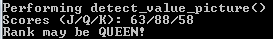
\includegraphics[width=0.6\textwidth]{chris/image27}
				\caption{Console output shows percentage match in clear favour of a Queen rank classification.}
				\label{fig:console}
			\end{figure}

			This entire process is shown in the implementation segment below (abbreviated):

			\begin{lstlisting}

//Load original SEs
cv::Mat se_symbols[3] = {
	cv::imread("res/symbols/scale_full/jack.png", CV_LOAD_IMAGE_GRAYSCALE),
	cv::imread("res/symbols/scale_full/queen.png", CV_LOAD_IMAGE_GRAYSCALE),
	cv::imread("res/symbols/scale_full/king.png", CV_LOAD_IMAGE_GRAYSCALE)
};

//Calculate new size
cv::Size size(100, 100);
cv::resize(mat_rank_1c, mat_rank_1c, size); //Should always be resized at runtime

//For reach symbol, resize SE
for(int j = 0; j < 3; j++)
{
	//Resize SE
	cv::resize(se_symbols[j], se_symbols[j], size); 
}

//Do matches using colour info integration
matches[JACK] += (int)round(hit_or_miss_score(mat_rank_1c, se_symbols[JACK]) * 100.0F);
matches[QUEEN] += (int)round(hit_or_miss_score(mat_rank_1c, se_symbols[QUEEN]) * 100.0F);
matches[KING] += (int)round(hit_or_miss_score(mat_rank_1c, se_symbols[KING]) * 100.0F);

cv::imshow("input", mat_rank_1c);
cv::imshow("template", se_symbols[QUEEN]);  //Only relevant for threecards.jpg

cout << "Scores (J/Q/K): " << matches[JACK] << "/" << matches[QUEEN] << "/" << matches[KING] << endl;

//Find which suit was matched most
if(max(matches[JACK], matches[QUEEN], matches[KING]) == matches[JACK])
{
	cout << "Rank may be JACK!" << endl;
	card->detected_rank = Card::RANK_JACK;
}
else if(max(matches[QUEEN], matches[QUEEN], matches[KING]) == matches[QUEEN])
{
	cout << "Rank may be QUEEN!" << endl;
	card->detected_rank = Card::RANK_QUEEN;
}
else if(max(matches[KING], matches[QUEEN], matches[KING]) == matches[KING])
{
	cout << "Rank may be KING!" << endl;
	card->detected_rank = Card::RANK_KING;
}
else
{
	cout << "No winner! UNKNOWN SUIT" << endl;
	card->detected_suit = Card::UNKNOWN_SUIT;
}
			\end{lstlisting}

		\subsubsection{Custom HoM Implementation}
			Mathematical Morphology operations are available as part of the OpenCV library (\code{cv::morphologyEx()}), but as a result of study of the theory and experimental requirements it was felt that a custom implementation of the theory was appropriate. This allows additional modification and parameterisation of the behaviour of required morphological operators. To this end the implementation uses the \code{binary_operation()}, \code{binary_closing()} and \code{hit_or_miss()} functions whose core workings are detailed below:

			A binary morphological erosion or dilation is performed on a pixel by pixel basis, with each pixel in the input image used as the centre of a symmetrical structuring element. In the case of erosion, the lowest value (any 0s) is set at the output pixel. In the case of dilation the greatest value (any 255s) is set as the output pixel. This is shown in the code segment below:

			\begin{lstlisting}

//For all X x Y pixels
int result = 0;
for(int y = 0; y < input.rows; y++)
{
	for(int x = 0; x < input.cols; x++)
	{
		//Reset for new neighbourhood
		result = 0;
			
		//Get local values
		bool break_now = false;
		for(int j = 0; j < element_size; j++)
		{
			for(int i = 0; i < element_size; i++)
			{
				//If in the image
				if(is_in_image((x - half) + i, (y - half) + j, input.cols, input.rows))
				{
					//Channel values
					int p = data[((y - half) + j) * input.step + ((x - half) + i) * input_channels];

					//Save brightest of that area
					if(mode == MODE_BINARY_DILATION)
					{
						if(p  > 128.0F) //Assuming binary input
						{
							result = 255;
							break_now = true;
							break;
						}
					}
					else
					{
						if(p < 128.0F)
						{
							result = 0;
							break_now = true;
							break;
						}
						else
						{
							result = 255;
						}
					}
				}
			}

			if(break_now == true)   //This is used for speed. Eg for erosion, if any are black, all become black
			{
				break;
			}
		}
	
		//Save output Mat data
		out_data[y * output.step + x * output_channels] = result;
	}
}
			\end{lstlisting}

			The end result of this operation is a \code{cv::Mat} containing an eroded or dilated image, depending on the mode passed as an argument. 

			The \code{binary_opening()} and \code{binary_closing()} functions simply chain calls to \code{binary_operation()} to implement the order of operations required for each operator. The example of \code{binary_closing()} is shown below:

			\begin{lstlisting}

cv::Mat binary_closing(cv::Mat input, int element_size)
{
	cout << "Performing binary closing..." << endl;

	cv::Mat working = input.clone();
	working = binary_operation(working, MODE_BINARY_DILATION, element_size);
	working = binary_operation(working, MODE_BINARY_EROSION, element_size);
	return working;
}
			\end{lstlisting}

			Finally, the morphological Hit-or-Miss transform is implemented by comparing all pixels in an input image to those in the equivalent locations in the structuring element image. Once all pixels have been compared, the total number of matched pixels is compared against a minimum to count as a match. In the case of \code{hit_or_miss_score()} the raw percentage of matched pixels is output as the return value. The implementation in code is shown below:

			\begin{lstlisting}

//For each position, try and find a match
int matched_pixels = 0;

//Search whole SE
for(int j = 0; j < img.rows; j++)
{
	for(int i = 0; i < img.cols; i++)
	{
		//Input pixel value
		int in_p = in_data[j * img.step + i * in_channels];
		int se_p = se_data[j * img.step + i * se_channels];

		//Minithresh - but should be binary anyway!
		in_p = in_p > 128 ? 255 : 0;
		se_p = se_p > 128 ? 255 : 0;

		if(in_p == se_p)
		{
			//Matching pixel found!
			matched_pixels++;
		}
	}
}

//Was this a matched template?
int total_pixels = img.rows * img.cols;
return (float)matched_pixels / (float)total_pixels;
			\end{lstlisting}

			This return value is then used to compare multiple structuring elements in the picture card rank finding as well as the suit symbol detection functions.